% ============================ 02 引导训练 ============================

\section{引导训练：代价梯度的传递机制}

\begin{frame}[plain]
  \begin{center}
    \vspace{1.2cm}
    {\color{yopoblue}\Huge\bfseries 02}\\[0.5em]
    {\color{yopoblue}\LARGE 引导训练：代价梯度的传递机制}\\[1.2em]
    \begin{minipage}{0.76\textwidth}
      \small\color{yopogray}
      训练阶段的评价环节并非学习得到的专家模型，而是由代价函数与特权地图查询构成的数值计算过程：
      给定候选的终端状态，返回代价 $J$ 与该终端状态的梯度；
      再由链式法则将其传递至网络权重。
    \end{minipage}
  \end{center}
\end{frame}

% ---------------------------------------------------------------
\begin{frame}{三种学习范式的比较}
  \begin{columns}[c]
    \begin{column}{0.55\textwidth}
      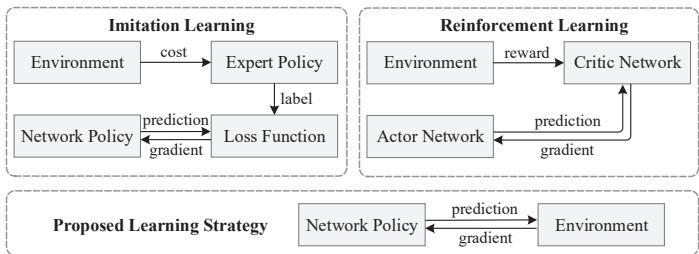
\includegraphics[width=\linewidth]{figures/02_learning_paradigms.jpg}
      \begin{center}\scriptsize\color{yopogray}
      原文 Fig.~2：模仿学习 / 强化学习 / 本文策略的对照
      \end{center}
    \end{column}
    \begin{column}{0.43\textwidth}
      \small
      \begin{itemize}\tight
        \item \textbf{模仿学习}：环境 $\to$ 专家 $\to$ 标签 $\to$ 损失；
              网络的上界就是专家。
        \item \textbf{强化学习}：环境给奖励 $\to$ 训练 Critic 来近似可导函数；
              奖励稀疏、需要大量交互。
        \item \textbf{引导学习}：环境\textbf{直接}给出可求导的代价——
              省掉中间那层近似。
      \end{itemize}
      \begin{reading}[关键区别]
        \small
        YOPO 认为规划问题的本质就是\textbf{梯度优化}。
        既然代价能求梯度，就没有必要先训一个 Critic 来假装它可导。
      \end{reading}
    \end{column}
  \end{columns}
\end{frame}

% ---------------------------------------------------------------
\begin{frame}{不同训练范式的代价分布对比}
  \small
  \begin{columns}[t]
    \begin{column}{0.6\textwidth}
      \begin{center}
      \begin{tabular}{@{}cc@{}}
        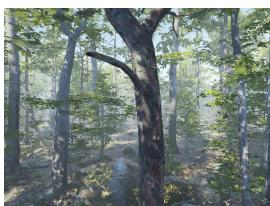
\includegraphics[width=0.36\linewidth]{figures/05a_simulated_scene.jpg} &
        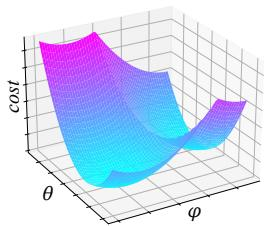
\includegraphics[width=0.36\linewidth]{figures/05b_wta_cost.jpg}\\
        \scriptsize (a) 仿真场景 &
        \scriptsize (b) Winner-Takes-All 代价 \\[3pt]
        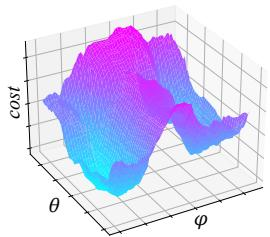
\includegraphics[width=0.36\linewidth]{figures/05c_critic_cost.jpg} &
        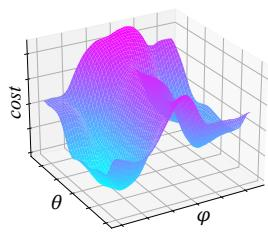
\includegraphics[width=0.36\linewidth]{figures/05d_realistic_cost.jpg}\\
        \scriptsize (c) Critic 网络给出的代价 &
        \scriptsize (d) 真实代价 \\
      \end{tabular}
      \end{center}
    \end{column}
    \begin{column}{0.38\textwidth}
      \scriptsize
      \begin{itemize}\tight
        \item \textbf{(b) 监督/模仿}：距离标签的二次型——
              一个光滑的碗，\textbf{没有多模态结构}。
        \item \textbf{(c) Critic}：训练不足时\textbf{噪声大}、曲面不平滑。
        \item \textbf{(d) 真实代价}：来自 ESDF 与运动学，
              有起伏、有多个局部极小——\textbf{这才是要拟合的目标}。
      \end{itemize}
      \begin{reading}
        \scriptsize
        原文 Fig.~5：固定当前状态、规划时域与终端导数，
        把 $\varphi,\theta$ 当自由变量画出的代价分布。
        把代价简化成“离标签多远”，信息量远不如直接使用规划代价本身。
      \end{reading}
    \end{column}
  \end{columns}
\end{frame}

% ---------------------------------------------------------------
\begin{frame}{引导学习：以数值梯度作为监督信号}
  \small
  \begin{columns}[t]
    \begin{column}{0.5\textwidth}
      \begin{block}{传统梯度优化的做法}
        \footnotesize
        查 ESDF 得到数值梯度 $\partial J/\partial(\text{轨迹参数})$，
        直接\textbf{更新轨迹参数}（多项式路点或 B 样条控制点）。
      \end{block}
      \begin{block}{YOPO 多做了一步}
        \footnotesize
        把这同一个数值梯度，\textbf{继续沿链式法则反传}
        到“生成这些轨迹参数的网络权重”。
      \end{block}
      \begin{paperfinding}[原文的三点理由]
        \footnotesize
        反馈\textbf{真实}（就是规划代价本身）、\textbf{准确}（不是近似目标）、
        \textbf{及时}（无需与环境反复交互）。
      \end{paperfinding}
    \end{column}
    \begin{column}{0.46\textwidth}
      \begin{teach}[两种更新对象的对照]
        \small
        \begin{tabular}{@{}p{0.44\linewidth}p{0.46\linewidth}@{}}
          \toprule
          传统优化器 & YOPO 训练 \\
          \midrule
          更新\newline 轨迹变量 $\mathbf q$ &
          更新\newline \textbf{生成 $\mathbf q$ 的网络权重} \\
          \addlinespace
          每条轨迹\newline 各自迭代 &
          共享权重\newline 一次反传覆盖 15 条 \\
          \addlinespace
          用最优解 & 用\textbf{代价梯度方向}，不必先给出唯一最优解 \\
          \bottomrule
        \end{tabular}
      \end{teach}
    \end{column}
  \end{columns}
\end{frame}

% ---------------------------------------------------------------
\begin{frame}{代价函数的构成}
  \small
  \begin{columns}[t]
    \begin{column}{0.5\textwidth}
      原文式 (10)：
      \[
        J=\lambda_sJ_s+\lambda_oJ_o+\lambda_gJ_g
      \]
      \begin{itemize}\tight
        \item $J_s$：平滑项，约束导数的平方积分；
        \item $J_o$：避障项，对靠近障碍施加惩罚；
        \item $J_g$：目标项，牵引朝向目标。
      \end{itemize}
      \begin{reading}[“真实代价”的含义]
        \small
        指\textbf{按设定的规划目标与训练环境直接计算}的值，
        并不是实际闭环飞行长期收益或安全性的完整真值。
      \end{reading}
    \end{column}
    \begin{column}{0.46\textwidth}
      \begin{block}{三个子问题}
        \footnotesize
        \begin{tabular}{@{}p{0.32\linewidth}p{0.6\linewidth}@{}}
          \toprule
          项 & 是否可解析求导 \\
          \midrule
          平滑 $J_s$ & \textbf{能}：轨迹是多项式，
                       代价可写成边界状态的二次型，梯度是闭式 \\
          \addlinespace
          目标 $J_g$ & \textbf{能}：终端位置的平方距离，梯度 $2(\mathbf p_T-\mathbf g)$ \\
          \addlinespace
          避障 $J_o$ & \textbf{不能}：距离来自 ESDF，
                       只能查表 + 差分，再按链式法则拼出梯度 \\
          \bottomrule
        \end{tabular}
      \end{block}
      \begin{reading}
        \scriptsize
        该区分与后文 $\partial J/\partial\mathbf q$ 的构成对应：
        三项中只有避障项依赖地图查询，因此该项梯度为数值形式。
      \end{reading}
    \end{column}
  \end{columns}
\end{frame}

% ---------------------------------------------------------------
\begin{frame}{边界状态的固定块与自由块分解}
  \small
  \begin{columns}[t]
    \begin{column}{0.52\textwidth}
      原文式 (11)：用选择矩阵 $C$ 把边界状态拆开
      \[
        \mathbf A=M^{-1}C\begin{bmatrix}\mathbf d_F\\ \mathbf d_P\end{bmatrix}
      \]
      \begin{itemize}\tight
        \item $\mathbf d_F$：\textbf{固定块}——当前状态（起点），来自状态估计，不可改；
        \item $\mathbf d_P$：\textbf{自由块}——终端状态，由网络预测，是待优化的量。
      \end{itemize}
      \begin{paperfinding}[与经典方法的差别]
        \small
        经典方法常在\textbf{固定终点}的前提下优化分段多项式；
        这里固定的是\textbf{时间 $T$}，
        优化的是\textbf{单段多项式的自由终点}。
      \end{paperfinding}
    \end{column}
    \begin{column}{0.44\textwidth}
      \begin{teach}[该拆分的意义]
        \small
        拆分之后，代价就变成“$\mathbf d_F$ 与 $\mathbf d_P$ 的二次型”，
        而网络只需要对 $\mathbf d_P$ 负责。
        于是 $\partial J/\partial\mathbf d_P$ 就是需要反传给网络的那一份梯度，
        $\partial J/\partial\mathbf d_F$ 不需要——起点不是网络产生的。
      \end{teach}
    \end{column}
  \end{columns}
\end{frame}

% ---------------------------------------------------------------
\begin{frame}{平滑项：二次型形式与解析梯度}
  \small
  \begin{columns}[t]
    \begin{column}{0.54\textwidth}
      原文式 (12)(13)：把 $\mathbf c^T M^{-T}QM^{-1}C$ 记作 $B$，则
      \[
        J_s=
        \begin{bmatrix}\mathbf d_F\\ \mathbf d_P\end{bmatrix}^{\!\mathsf T}
        \begin{bmatrix}B_{FF}&B_{FP}\\ B_{PF}&B_{PP}\end{bmatrix}
        \begin{bmatrix}\mathbf d_F\\ \mathbf d_P\end{bmatrix}
      \]
      原文式 (14)：对自由块求导
      \[
        \frac{\partial J_s}{\partial\mathbf d_P}
        =2\,\mathbf d_F^{\mathsf T}B_{FP}+2\,\mathbf d_P^{\mathsf T}B_{PP}
      \]
      \begin{reading}[闭式梯度的来源]
        \scriptsize
        轨迹参数对边界条件是\textbf{线性}的（$\mathbf c=M^{-1}\mathbf d$），
        而导数的平方积分对系数是\textbf{二次}的。
        线性变换代入二次型 $\Rightarrow$ 对边界条件仍是二次型，
        梯度自然是线性表达式。
      \end{reading}
    \end{column}
    \begin{column}{0.42\textwidth}
      \begin{block}{矩阵的角色}
        \footnotesize
        \begin{tabular}{@{}ll@{}}
          \toprule
          $M^{-1}$ & 边界条件 $\to$ 多项式系数 \\
          $Q$ & 导数平方积分的二次型核 \\
          $C$ & 选出自由块 \\
          $B$ & 合成后的“代价矩阵” \\
          \bottomrule
        \end{tabular}
      \end{block}
      \begin{reading}[用哪一阶导数]
        \small
        原文实验采用\textbf{ jerk（三阶导）平方的积分}衡量平滑性，
        与论文对平滑度的定义一致。
        具体阶次、权重与归一化仍应对照所引用的版本。
      \end{reading}
    \end{column}
  \end{columns}
\end{frame}

% ---------------------------------------------------------------
\begin{frame}{避障项：势函数与时间积分}
  \small
  \begin{columns}[t]
    \begin{column}{0.5\textwidth}
      原文式 (15)：把安全代价定义为势函数沿轨迹的\textbf{时间积分}，
      并离散化求和
      \[
        J_o=\int_0^{T}c(\mathbf p(t))\,dt
        \;\approx\;\sum_{\kappa=0}^{T/\delta t}c(\mathbf p(\mathcal T_\kappa))\,\delta t
      \]
      原文式 (16)：势函数取指数形式
      \[
        c(d_t)=\exp\!\Bigl(-\frac{d_t-d_0}{k}\Bigr)
      \]
      $d_t$ 为最近障碍距离，$d_0,k$ 为预设尺度参数。
    \end{column}
    \begin{column}{0.46\textwidth}
      \begin{center}
      \begin{tikzpicture}[x=0.9cm,y=0.55cm,every node/.style={font=\scriptsize}]
        \draw[->] (0,0) -- (4.6,0) node[right]{距离 $d_t$};
        \draw[->] (0,0) -- (0,2.6) node[above]{$c(d_t)$};
        \draw[thick,yopoorange,domain=0:4.4,samples=60] plot (\x,{2.3*exp(-(\x-0.6)/0.9)});
        \draw[dashed,yopogray] (0.6,0) -- (0.6,2.3);
        \node[below,color=yopogray] at (0.6,0) {$d_0$};
        \node[color=yopoorange] at (3.2,1.1) {离障碍越近，代价越大};
      \end{tikzpicture}
      \end{center}
      \vspace{-0.4em}
      \begin{paperfinding}[采用时间积分的理由]
        \footnotesize
        若用线积分，无人机会通过\textbf{缩短路程}来降低累计代价，产生“抄近道穿过障碍”的偏差。
        固定时间、自由终点的设置下，时间积分消除了这个偏差。
      \end{paperfinding}
    \end{column}
  \end{columns}
\end{frame}

% ---------------------------------------------------------------
\begin{frame}{避障项：梯度计算}
  \small
  \begin{columns}[t]
    \begin{column}{0.52\textwidth}
      原文式 (17)：离散形式的雅可比
      \[
        \frac{\partial J_o}{\partial\mathbf d_{P\mu}}
        =\sum_{\kappa=0}^{T/\delta t}
        \nabla_\mu c\bigl(\mathbf p(\mathcal T_\kappa)\bigr)\,
        \mathbf T\,\mathbf L_P\,\delta t
      \]
      该式即标准的链式相乘，两项分别对应：

      \vspace{0.3em}
      \begin{center}
      \begin{tikzpicture}[node distance=4mm,every node/.style={font=\scriptsize,align=center}]
        \node[draw=yopogreen,fill=yopopale,rounded corners,inner sep=3pt] (p) {采样点位置\\$\partial\mathbf p(t_\kappa)/\partial\mathbf d_P$};
        \node[draw=yopoorange,fill=yopowarm,rounded corners,inner sep=3pt,right=of p] (c) {势函数梯度\\$\nabla c$};
        \draw[-{Latex},thick] (p)--(c);
      \end{tikzpicture}
      \end{center}
      \vspace{-0.2em}
      写成更直白的形式：
      \[
        \frac{\partial J_o}{\partial\mathbf q}
        \approx\sum_\kappa
        \Bigl(\frac{\partial\mathbf p(t_\kappa)}{\partial\mathbf q}\Bigr)^{\!\mathsf T}
        \nabla_{\mathbf p}c\;\delta t
      \]
    \end{column}
    \begin{column}{0.44\textwidth}
      \begin{block}{两项的来源}
        \footnotesize
        \begin{itemize}\tight
          \item $\partial\mathbf p(t_\kappa)/\partial\mathbf q$：
                \textbf{解析可算}——多项式对边界条件是线性的，
                在时刻 $t_\kappa$ 处就是幂次基 $\times\,L_P$；
          \item $\nabla_{\mathbf p}c=-c\,\nabla_{\mathbf p}d/k$：
                \textbf{必须查地图}——$d$ 与其梯度来自 ESDF，
                地图查询通常无法被深度学习框架自动微分。
        \end{itemize}
      \end{block}
      \begin{reading}[实现上的做法]
        \small
        在采样点上取距离与距离梯度，\textbf{外部算出}数值梯度后，
        再按上面的链式关系拼成对终端状态的梯度。
      \end{reading}
    \end{column}
  \end{columns}
\end{frame}

% ---------------------------------------------------------------
\begin{frame}{目标项：临时目标点的构造}
  \small
  \begin{columns}[t]
    \begin{column}{0.5\textwidth}
      原文式 (18)(19)：把最终目标投影到无人机周围\textbf{固定半径球面}上，
      得到一个临时目标 $\mathbf g$，
      \[
        J_g=\lVert \mathbf p_T-\mathbf g\rVert^2,\qquad
        \frac{\partial J_g}{\partial\mathbf p_T}=2(\mathbf p_T-\mathbf g)
      \]
      梯度就是“从当前终端点到临时目标的向量”。
    \end{column}
    \begin{column}{0.46\textwidth}
      \begin{reading}[临时目标投影的作用]
        \small
        目标可能在几十米外，而规划时域只有 $2$\,s。
        直接使用远处的最终目标，会让 $J_g$ 数值巨大、把另外两项压没，
        \textbf{数值不稳定}。
        投影到固定半径球面后，目标项与规划尺度匹配，
        同时仍然表达“朝那个方向走”的意图。
      \end{reading}
      \begin{reading}[两个“目标”记号的区分]
        \scriptsize
        $\hat{\mathbf g}$ 是\textbf{网络输入}的目标单位方向（只有方向）；
        $\mathbf g_{\mathrm{local}}$ 是\textbf{代价函数}里的临时目标点（有距离）。
        二者记号必须分开。
      \end{reading}
    \end{column}
  \end{columns}
\end{frame}

% ---------------------------------------------------------------
\begin{frame}{链式法则：外部梯度到网络权重的传递}
  \small
  \begin{center}
  \begin{tikzpicture}[node distance=6mm,every node/.style={font=\scriptsize,align=center}]
    \node[draw=yopoblue,fill=yopopale,rounded corners,inner sep=4pt] (w) {网络权重 $\mathbf w$};
    \node[draw=yopoblue,fill=yopopale,rounded corners,inner sep=4pt,right=of w] (y) {原始输出 $\mathbf y$\\(每格 10 个数)};
    \node[draw=yopoblue,fill=yopopale,rounded corners,inner sep=4pt,right=of y] (q) {终端状态 $\mathbf q$\\(15 组 $\times$ 9)};
    \node[draw=yopoorange,fill=yopowarm,rounded corners,inner sep=4pt,right=of q] (J) {轨迹代价 $J$\\(多项式重建 + ESDF)};

    \draw[-{Latex},thick] (w)--(y);
    \draw[-{Latex},thick] (y)--(q);
    \draw[-{Latex},thick] (q)--(J);
    \node[above=1mm of y,color=yopogray,font=\tiny]{前向：普通张量计算};
    \node[above=1mm of J,color=yopogray,font=\tiny]{前向：外部数值计算};

    \draw[-{Latex},thick,yopoorange] ($(J.south)+(0,-0.55)$) -- ($(q.south)+(0,-0.55)$);
    \draw[-{Latex},thick,yopoorange] ($(q.south)+(0,-0.55)$) -- ($(y.south)+(0,-0.55)$);
    \draw[-{Latex},thick,yopoorange] ($(y.south)+(0,-0.55)$) -- ($(w.south)+(0,-0.55)$);
    \node[below=1mm of q,yshift=-4mm,color=yopoorange,font=\tiny]{反向：链式相乘};
  \end{tikzpicture}
  \end{center}
  \vspace{-0.2em}
  原文式 (20) 就是这条反向路径的数学写法：
  \[
    \begin{aligned}
      \frac{\partial J}{\partial y_\epsilon}
      &=\underbrace{\frac{\partial J}{\partial\mathbf d_P}}_{\text{外部数值梯度}}
       \cdot\underbrace{\frac{\partial\mathbf d_P}{\partial\Delta\epsilon}}_{\text{球坐标解码}}
       \cdot\underbrace{\frac{\partial\Delta\epsilon}{\partial y_\epsilon}}_{\tanh}\\[2pt]
      \frac{\partial J}{\partial y_\varepsilon}
      &=\frac{\partial J}{\partial\mathbf d_P}\cdot
        \frac{\partial\mathbf d_P}{\partial y_\varepsilon}
    \end{aligned}
    \qquad(\epsilon\in\{\theta,\varphi,r\},\;\varepsilon\in\{v,a\})
  \]
  \begin{reading}[自定义 autograd 层的接口位置]
    \scriptsize
    PyTorch 无法对 $J$ 的计算过程自动求导。
    实现上用自定义 autograd 函数封装评价器：
    前向返回代价，反向\textbf{直接返回外部算出的 $\partial J/\partial\mathbf q$}。
    该层之后即为标准反向传播。
  \end{reading}
\end{frame}

% ---------------------------------------------------------------
\begin{frame}{轨迹与评分的两条梯度路径}
  \begin{columns}[c]
    \begin{column}{0.58\textwidth}
      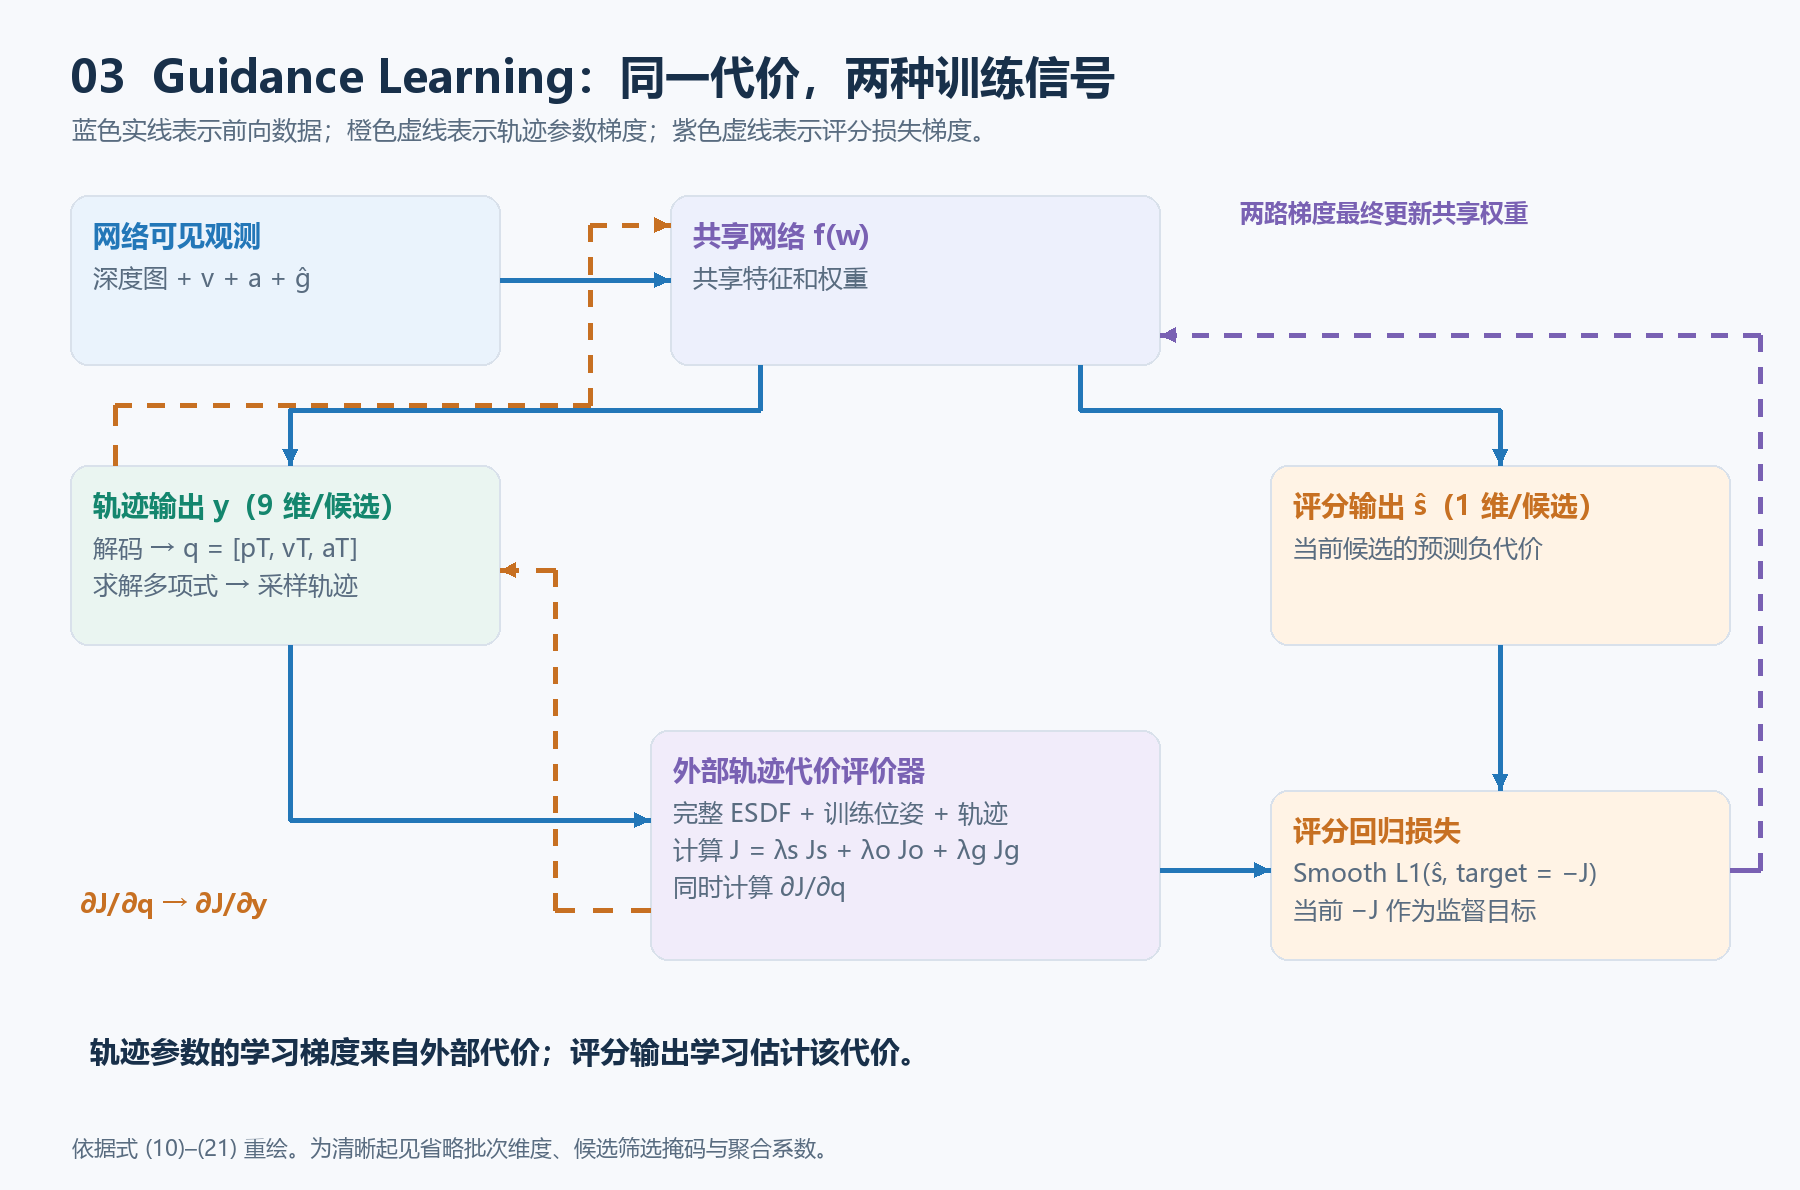
\includegraphics[width=\linewidth]{figures/22_note_training_gradients.png}
      \begin{center}\scriptsize\color{yopogray}
      笔记图 3：蓝色为前向数据流，橙色为轨迹参数梯度，
      紫色为评分损失梯度
      \end{center}
    \end{column}
    \begin{column}{0.4\textwidth}
      \small
      \begin{block}{路径一：轨迹参数}
        \footnotesize
        外部代价梯度 $\partial J/\partial\mathbf q$
        $\to$ 解码链 $\partial\mathbf q/\partial\mathbf y$
        $\to$ 共享网络权重。
        \textbf{这条路径不经过预测评分}——
        轨迹不是靠“评分告诉它该往哪改”来改进的。
      \end{block}
      \begin{block}{路径二：评分}
        \footnotesize
        预测评分与“当前候选的负代价”之间的回归误差，
        直接反向传播到评分通道（也会经共享骨干影响特征）。
      \end{block}
      \begin{reading}
        \scriptsize
        两条路径最终作用于\textbf{同一组权重}，
        因此是共同优化，而不是两个互不影响的网络。
      \end{reading}
    \end{column}
  \end{columns}
\end{frame}

% ---------------------------------------------------------------
\begin{frame}{评分输出的学习目标}
  \small
  \begin{columns}[t]
    \begin{column}{0.5\textwidth}
      原文式 (21)：轨迹评分定义为 $-J$，用 smooth $L_1$ 监督
      \[
        \mathcal L=\text{Smooth}L_1\bigl(y_s,\,-J\bigr)
      \]
      \begin{itemize}\tight
        \item $y_s$：网络预测的评分（共享特征上的第 10 个输出）；
        \item $-J$：由评价器\textbf{当场算出}的目标；
        \item 两者误差经普通反向传播回到评分通道。
      \end{itemize}
      \begin{paperfinding}[在线如何使用]
        \footnotesize
        部署时没有地图，无法计算 $J$，
        于是用预测评分代替真实的代价排序——
        选评分最高的候选（等价于代价最低）。
      \end{paperfinding}
    \end{column}
    \begin{column}{0.46\textwidth}
      \begin{reading}[“评分是不是一个独立回归问题”]
        \small
        形式上是一个回归，但\textbf{不独立}，有三重耦合：
        \begin{itemize}\tight
          \item \textbf{目标不是固定标签}：目标由网络自己当前的输出算出，
                网络一变、标签就变；
          \item \textbf{梯度进同一个骨干}：评分误差会改变共享特征，
                从而改变下一轮的轨迹输出；
          \item \textbf{它是评分通道唯一的监督}：没有它，第 10 个输出学不会。
        \end{itemize}
        真正被切断的只有一条：评分误差\textbf{不能直接把终端状态改掉}。
      \end{reading}
    \end{column}
  \end{columns}
\end{frame}

% ---------------------------------------------------------------
\begin{frame}{评分学习：数值算例}
  \footnotesize
  \begin{columns}[c]
    \begin{column}{0.56\textwidth}
      \begin{teach}[构造的两条候选（三个权重都取 1）]
        \scriptsize
        \begin{tabular}{@{}lrr@{}}
          \toprule
          项目 & 候选 A & 候选 B \\
          \midrule
          平滑 $J_s$ & 0.10 & 0.20 \\
          避障 $J_o$ & 0.70 & 0.05 \\
          目标 $J_g$ & 0.20 & 0.15 \\
          \midrule
          合计 $J$ & 1.00 & \textbf{0.40} \\
          目标 $-J$ & $-1.00$ & $-0.40$ \\
          当前预测 $\hat s$ & $-0.20$ & $-0.90$ \\
          \bottomrule
        \end{tabular}
      \end{teach}
      \begin{reading}
        \scriptsize
        当前预测会选 A，但按评价器应选 \textbf{B}——
        这正是评分误差要修正的排序错误。
        （论文实测：专家平均代价 0.078、网络训练后 0.050，
        候选间的代价差距远小于本表的教学数字。）
      \end{reading}
    \end{column}
    \begin{column}{0.4\textwidth}
      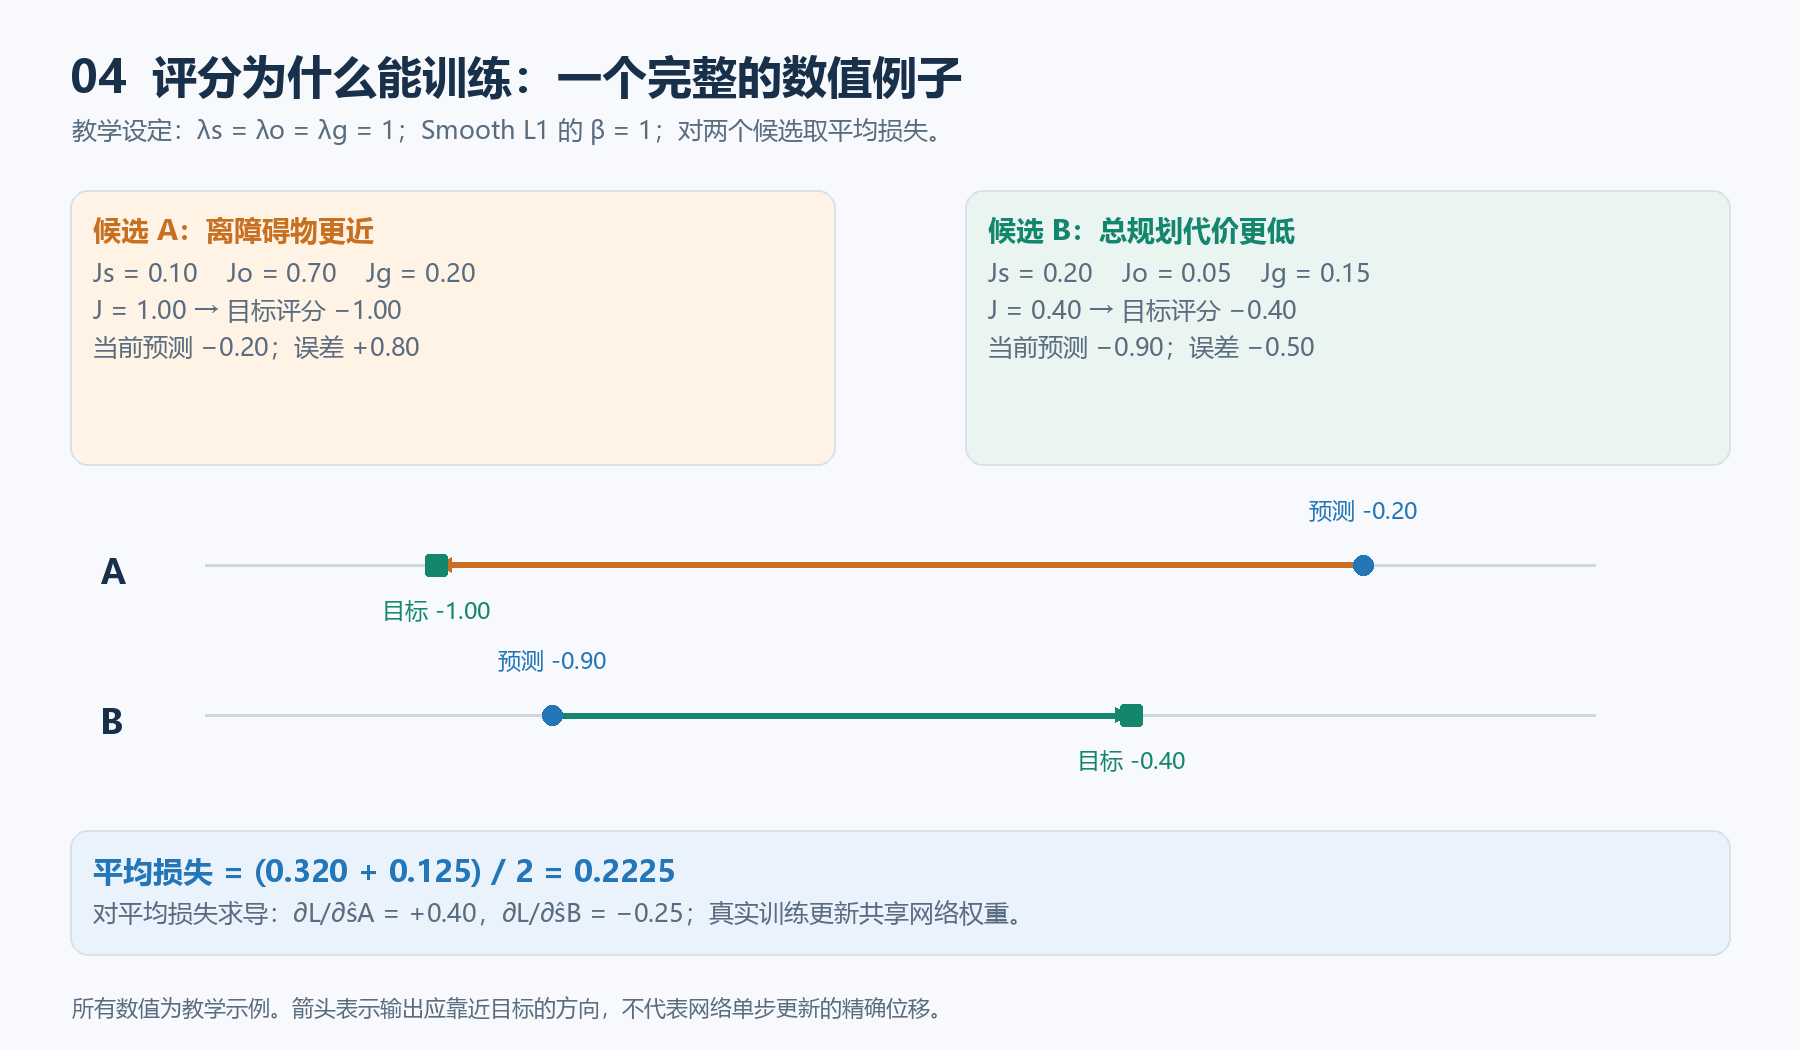
\includegraphics[width=\linewidth]{figures/23_note_score_learning.png}
      \begin{center}\scriptsize\color{yopogray}
      笔记图 4：蓝点为预测，绿方块为目标，
      箭头表示误差应减小的方向
      \end{center}
    \end{column}
  \end{columns}
\end{frame}

% ---------------------------------------------------------------
\begin{frame}{候选筛选策略}
  \small
  \begin{columns}[t]
    \begin{column}{0.5\textwidth}
      \begin{paperfinding}[原文的描述]
        \footnotesize
        \begin{itemize}\tight
          \item \textbf{所有}基元的预测评分都参与训练；
          \item 但只有\textbf{评分高于阈值}的候选，其终端状态才接受轨迹优化的训练；
          \item 实验阈值为 \textbf{0.04}；
          \item 阈值过小 $\to$ 过拟合到安全条件、整体不稳定；
                阈值过大 $\to$ 受负样本影响、难以收敛。
        \end{itemize}
      \end{paperfinding}
    \end{column}
    \begin{column}{0.46\textwidth}
      \begin{reading}[候选筛选的作用]
        \small
        代价很高的候选（例如直接朝向障碍）其梯度方向参考价值有限，
        让它参与“把终点往哪推”的学习可能引入噪声。
        因此：\textbf{评分继续学全部候选，轨迹参数只学可救的那部分}。
      \end{reading}
      \begin{reading}[记号方向的注意事项]
        \scriptsize
        原文把评分定义为 $-J$（越大越好），
        所以“评分高于阈值”与“代价低于阈值”是同一件事。
        阅读时需注意符号方向，避免误读为“训练代价最大的候选”。
      \end{reading}
    \end{column}
  \end{columns}
\end{frame}

% ---------------------------------------------------------------
\begin{frame}[shrink=6]{特权学习：训练与部署的信息差异}
  \begin{columns}[c]
    \begin{column}{0.62\textwidth}
      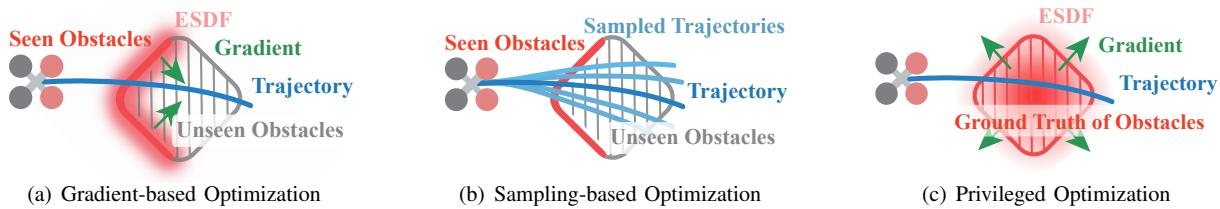
\includegraphics[width=0.94\linewidth]{figures/06_privileged_learning.jpg}
      \begin{center}\scriptsize\color{yopogray}
      原文 Fig.~6：(a) 梯度法、(b) 采样法、
      (c) 特权优化——前两者会被遮挡或初始值困住
      \end{center}
    \end{column}
    \begin{column}{0.36\textwidth}
      \small
      \begin{block}{训练时可访问}
        \footnotesize
        \begin{itemize}\tight
          \item 完整点云与 ESDF 地图；
          \item 无人机完整状态（位置、姿态）；
          \item 用于计算代价与梯度。
        \end{itemize}
      \end{block}
      \begin{block}{部署时只有}
        \footnotesize
        \begin{itemize}\tight
          \item 噪声深度图；
          \item 速度、加速度、目标方向；
          \item 状态估计给出的当前位置。
        \end{itemize}
      \end{block}
      \begin{reading}
        \scriptsize
        特权信息\textbf{不进入网络输入}，
        只用于产生监督。因此部署仍受有限视野与部分可观测性限制，
        但其学习信号来自完整环境。
      \end{reading}
    \end{column}
  \end{columns}
\end{frame}

% ---------------------------------------------------------------
\begin{frame}{数据与训练配置}
  \small
  \begin{columns}[t]
    \begin{column}{0.5\textwidth}
      \begin{block}{原文给出的训练设置}
        \footnotesize
        \begin{tabular}{@{}ll@{}}
          \toprule
          数据集 & Flightmare 中随机重置状态采集 \\
          样本量 & 约 \textbf{100K} \\
          迭代 & \textbf{50} 个 epoch \\
          批量大小 & \textbf{16} \\
          学习率 & $1.5\times10^{-4}$ \\
          优化器 & Adam \\
          无效深度 & 最近邻插值填充 \\
          进一步微调 & 数据聚合（DAgger）\\
          \bottomrule
        \end{tabular}
      \end{block}
    \end{column}
    \begin{column}{0.46\textwidth}
      \begin{paperfinding}[无需重新标注的原因]
        \small
        同一张深度图可以配\textbf{不同的速度、加速度与目标方向}，
        每次都重新计算代价即可——
        不需要重新生成专家轨迹标签，也不需要重新与仿真器交互。
        这是“无专家”带来的数据增广能力。
      \end{paperfinding}
      \begin{reading}[“无监督”的准确含义]
        \scriptsize
        不依赖\textbf{专家最优轨迹示范}，
        但依赖\textbf{人为设计的代价、环境特权信息}与\textbf{计算出的监督信号}。
        与“没有任何监督信号”不是一回事。
      \end{reading}
    \end{column}
  \end{columns}
\end{frame}

% ---------------------------------------------------------------
\begin{frame}{训练与推理的数据流对照}
  \scriptsize
  \begin{center}
  \begin{tabular}{@{}p{0.22\textwidth}p{0.335\textwidth}p{0.335\textwidth}@{}}
    \toprule
    \textbf{环节} & \textbf{训练阶段} & \textbf{在线推理阶段} \\
    \midrule
    网络输入 & 深度、速度、加速度、目标方向 & 相同类型的可观测输入 \\
    \addlinespace
    网络输出 & 15 组参数与评分 & 15 组参数与评分 \\
    \addlinespace
    候选轨迹求解 & 为计算代价与梯度，\textbf{15 条都要生成} & 只需求解\textbf{被选中的那一条} \\
    \addlinespace
    完整地图与位姿 & 供外部评价器计算代价与梯度 & 在线规划\textbf{不依赖}训练用完整 ESDF \\
    \addlinespace
    规划代价 $J$ & 直接计算并指导训练 & 用\textbf{预测评分}估计质量 \\
    \addlinespace
    反向传播 & 两种信号更新共享权重 & 无 \\
    \addlinespace
    控制器执行 & 主训练反馈\textbf{不要求}逐条闭环执行 & 跟踪选中轨迹、持续重规划 \\
    \bottomrule
  \end{tabular}
  \end{center}
  \vspace{0.2em}
  \begin{reading}
    \scriptsize
    需注意“候选轨迹求解”一行：
    训练时 15 条均需解出多项式方可计算代价，在线时仅求解 1 条。
  \end{reading}
\end{frame}
